\chapter{补充图表与统计分析示例}\label{app:appendixB}

本附录用于展示第二类补充材料的排版方式，例如额外统计结果、模型参数说明、补充流程图及原始图片等。附录 B 与附录 A 的图表编号独立连续，并保持与正文一致的题注样式。

\section{补充表格示例}

\begin{center}
	\captionof{table}[附录 B 中补充统计结果示例]{附录 B 中补充统计结果示例\par
		{\qauTimes\fontsize{10.5bp}{15.75bp}\selectfont \textbf{Table~\thetable\ Example of supplementary statistical results in Appendix B}}}
	\label{tab:appendix-b-stat}
	\renewcommand{\arraystretch}{1.5}
	{\songti\zihao{5}
		\begin{tabular*}{0.8\textwidth}{@{\extracolsep{\fill}}>{\centering\arraybackslash}m{0.18\textwidth}>{\centering\arraybackslash}m{0.26\textwidth}>{\centering\arraybackslash}m{0.26\textwidth}}
			\toprule
			{\songti\zihao{5}处理} & {\songti\zihao{5}指标 1} & {\songti\zihao{5}指标 2} \\
			\midrule
			CK & 0.00$\pm$0.00\textsuperscript{a} & 0.00$\pm$0.00\textsuperscript{a} \\
			T1 & 0.00$\pm$0.00\textsuperscript{b} & 0.00$\pm$0.00\textsuperscript{ab} \\
			T2 & 0.00$\pm$0.00\textsuperscript{c} & 0.00$\pm$0.00\textsuperscript{b} \\
			\bottomrule
		\end{tabular*}
	}
\end{center}

%\newpage

\section{补充图片示例}

\begin{center}
	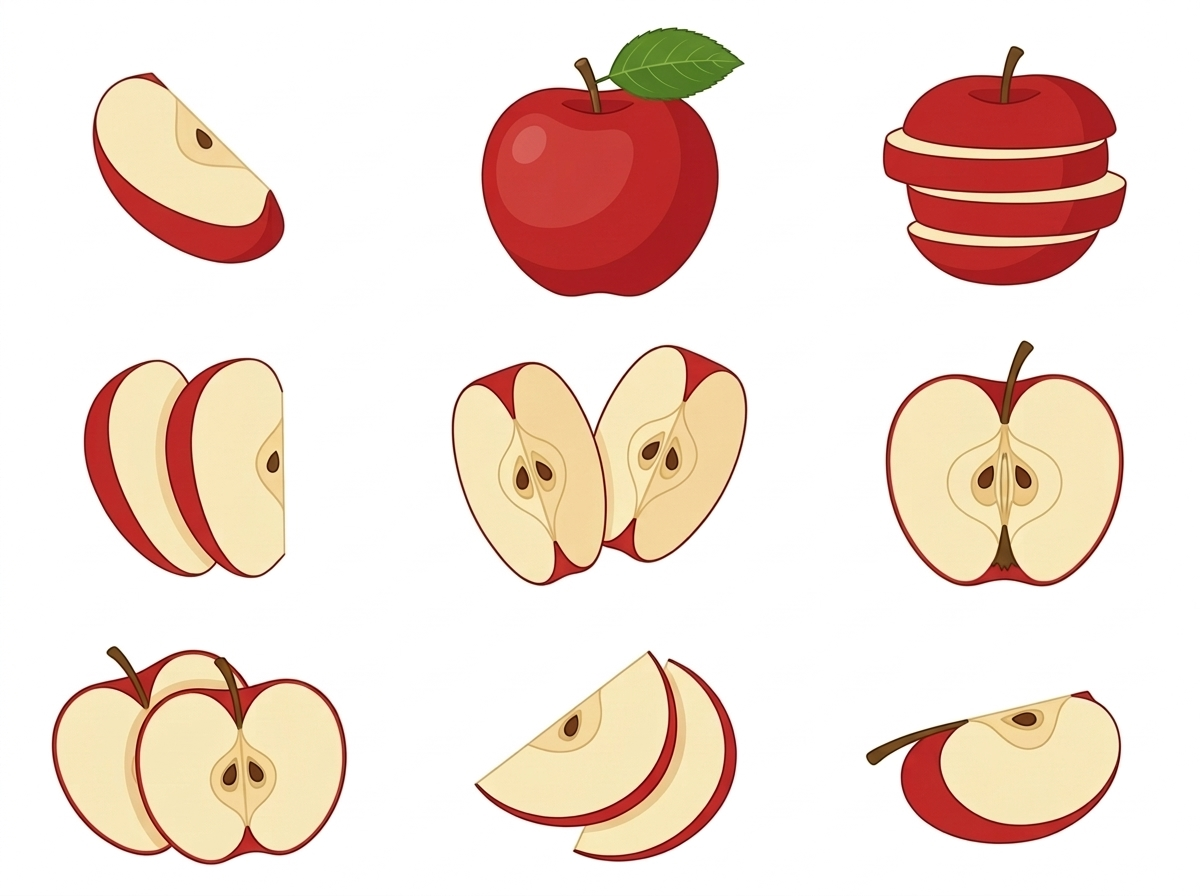
\includegraphics[width=0.45\textwidth]{figures/apple.png}
	\captionof{figure}[附录 B 中补充图片占位示例]{附录 B 中补充图片占位示例。\par
		（A）XXXX；（B）XXXX；（C）XXXX。\par
		注：不同小写字母代表存在显著差异（$p<0.05$）。\par
		{\qauTimes\fontsize{10.5bp}{15.75bp}\selectfont \textbf{Fig.~\thefigure\ Example of supplementary figure in Appendix B.}}\par
		{\qauTimes\fontsize{10.5bp}{15.75bp}\selectfont \textbf{(A) XXXX; (B) XXXX; (C) XXXX.}}\par
        {\qauTimes\fontsize{10.5bp}{15.75bp}\selectfont \textbf{Different lowercase letters indicate significant differences (\boldmath$p<0.05$).}}}
	\label{fig:appendix-b-figure}
\end{center}